\chapter{Exploring the Uncanny Valley in Human-Like Robot Recruiters}
\label{chap:6}
Human resource operations are progressively becoming more digital. Many procedures are already automated, and the use of artificial intelligence is also becoming increasingly common. Especially in the recruitment process, a new approach called robot recruiting is being applied. Robot recruitment describes a semi-automatic process in which algorithms and artificial intelligence take over parts of the typical recruiting process, such as assessing and selecting applicants \cite{vera}. By analysing vast amounts of data, these algorithms are trained to assist companies in making predictions and decisions on future employees \cite{robot_recruiting_scholar}. This assistance is hoped to shorten the time-consuming process of personnel recruitment and employ a more neutral way of evaluating the applicants \cite{robot_recruiting_scholar}.\\
Many people are already familiar with websites that provide a chat window where one can talk to supposed employees. Often these 'employees' are, in fact, algorithms with which you can communicate, and they can perform a variety of simple tasks \cite{vera}. These algorithms are among the best-known applications similar to the intention of robot recruiting. When applying this concept to the recruitment processes, an algorithm takes over the simpler communication and carries out sorting, admission and possibly an exclusion of applicants \cite{vera}. However, with the rapid development of information technology, robot recruiters can take on even more complex tasks, such as conducting a job interview \cite{vera}. For this task, however, the algorithms need a medium with which to communicate with candidates, and a human-like figure in the shape of an online character or a robot is frequently used for this purpose. One example of this is a Russian start-up which has developed a robot recruitment system called robot Vera, with which companies can conduct telephone interviews with applicants \cite{vera}. This robot recruiter talks to the applicants self-sufficiently and responds to their questions. During the telephone interview, the robot takes on a female human form \cite{vera}.
With the development of a human-like appearance of robot recruiters, the effect of the uncanny valley on them also becomes relevant. If the appearance of a robot recruiter falls into the uncanny valley, it could affect the applicant's acceptance of the recruiter during the interview. This could negatively impact the applicant's behaviour and, therefore, their performance during the application process.
With the help of an online survey based on rating potential robot recruiters with varying human-likeness, this thesis explores how applicants' feelings toward different designs of robot recruiters vary. With the survey results, the thesis then tries to determine if very but not perfectly human-like robot recruiters fall into the uncanny valley. The results are also used to make a recommendation for the aspired degree of human-likeness of such entities. 

\section{Stimuli}
For the survey, eight images \ref{fig:image-1} - \ref{fig:image-8} of possible robot recruiters with different degrees of human-likeness and a control image of a real human \ref{fig:image-9} were selected. When choosing the entities, special consideration was given to the fact that they either currently exist or may be plausible as a design for a robot recruiter. Among the images are four avatars that are currently in development or use. Figure \ref{fig:image-2} shows the existing robot recruiter, Tengai, a physical robot developed to assist recruiters and hiring managers. More information about the company and this robot recruiter can be found on the company's website (https://www.tengai-unbiased.com/tengai-robot/). Image \ref{fig:image-5} shows a design of the robot recruiter Vera, which is developed by a Russian start-up company \cite{vera}. Figure \ref{fig:image-3} shows an avatar of the Microsoft Mesh system, which is currently under development and aims to connect people working remotely in virtual space via Mixed Reality with the help of avatars \cite{microsoft_mesh}. Although this system was not specifically designed for robot recruiting, such a design could easily be imagined. Image \ref{fig:image-4} shows the humanoid robot Sophia, which was developed by the Hong Kong company Hanson Robotics. Sophia became internationally known due to its particularly human appearance and behaviour compared to previous robot variants. The remaining figures \ref{fig:image-1}, \ref{fig:image-6}, \ref{fig:image-7}, \ref{fig:image-8} were chosen to represent a broader range of human-likeness levels and to compare existing appearances to other possibilities. The images are ordered in ascending human-likeness, which was objectively assessed by using the Human-Likeness Predictor of the ABOT Database (https://www.abotdatabase.info/) and by the addition of the study's evaluation, which is discussed in the following sections. The constant values from figure \ref{fig:image-5} to \ref{fig:image-8} can be explained by the evaluation of the ABOT database, which in its current state only gives a rough assessment, and the variations in the human-likeness of the picked entities are already very modest.
\begin{table}[b!]
\centering
\resizebox{\linewidth}{!}{%
\begin{tabular}{ll|ll|ll}
\ref{fig:image-1} &Human-Likeness: 47.27 &\ref{fig:image-4} &Human-Likeness: 88.72 &\ref{fig:image-7} &Human-Likeness: 94.55 \\ \hline
\ref{fig:image-2} &Human-Likeness: 65.16 &\ref{fig:image-5} &Human-Likeness: 94.55 &\ref{fig:image-8} &Human-Likeness: 94.55 \\ \hline
\ref{fig:image-3} &Human-Likeness: 84.13 &\ref{fig:image-6} &Human-Likeness: 94.55 &\ref{fig:image-9} &Human-Likeness: 100
\end{tabular}
}
\caption{Rated human-likeness of the figures.}
\label{tab:rated-human-likeness}
\end{table}
\newpage

\begin{figure}[t!]
 \centering
 \subfloat[\cite{icup}\label{fig:image-1}]{%
      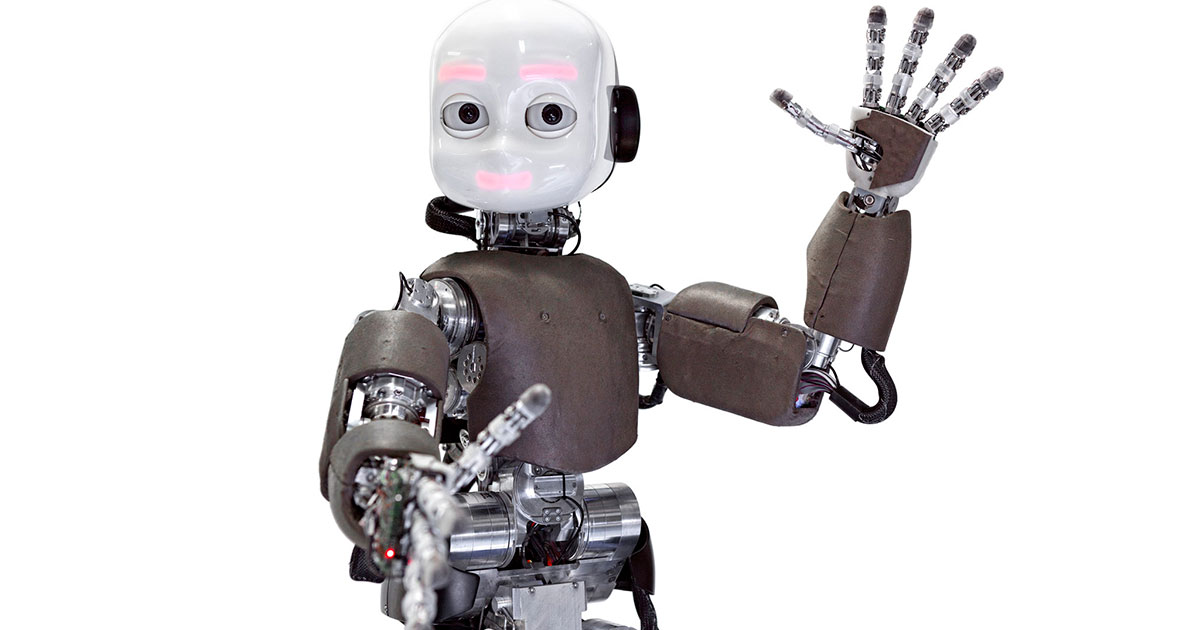
\includegraphics[width=0.26\textwidth]{graphics/study/icup.jpg}}
 \qquad
 \subfloat[\cite{tengai}\label{fig:image-2}]{%
      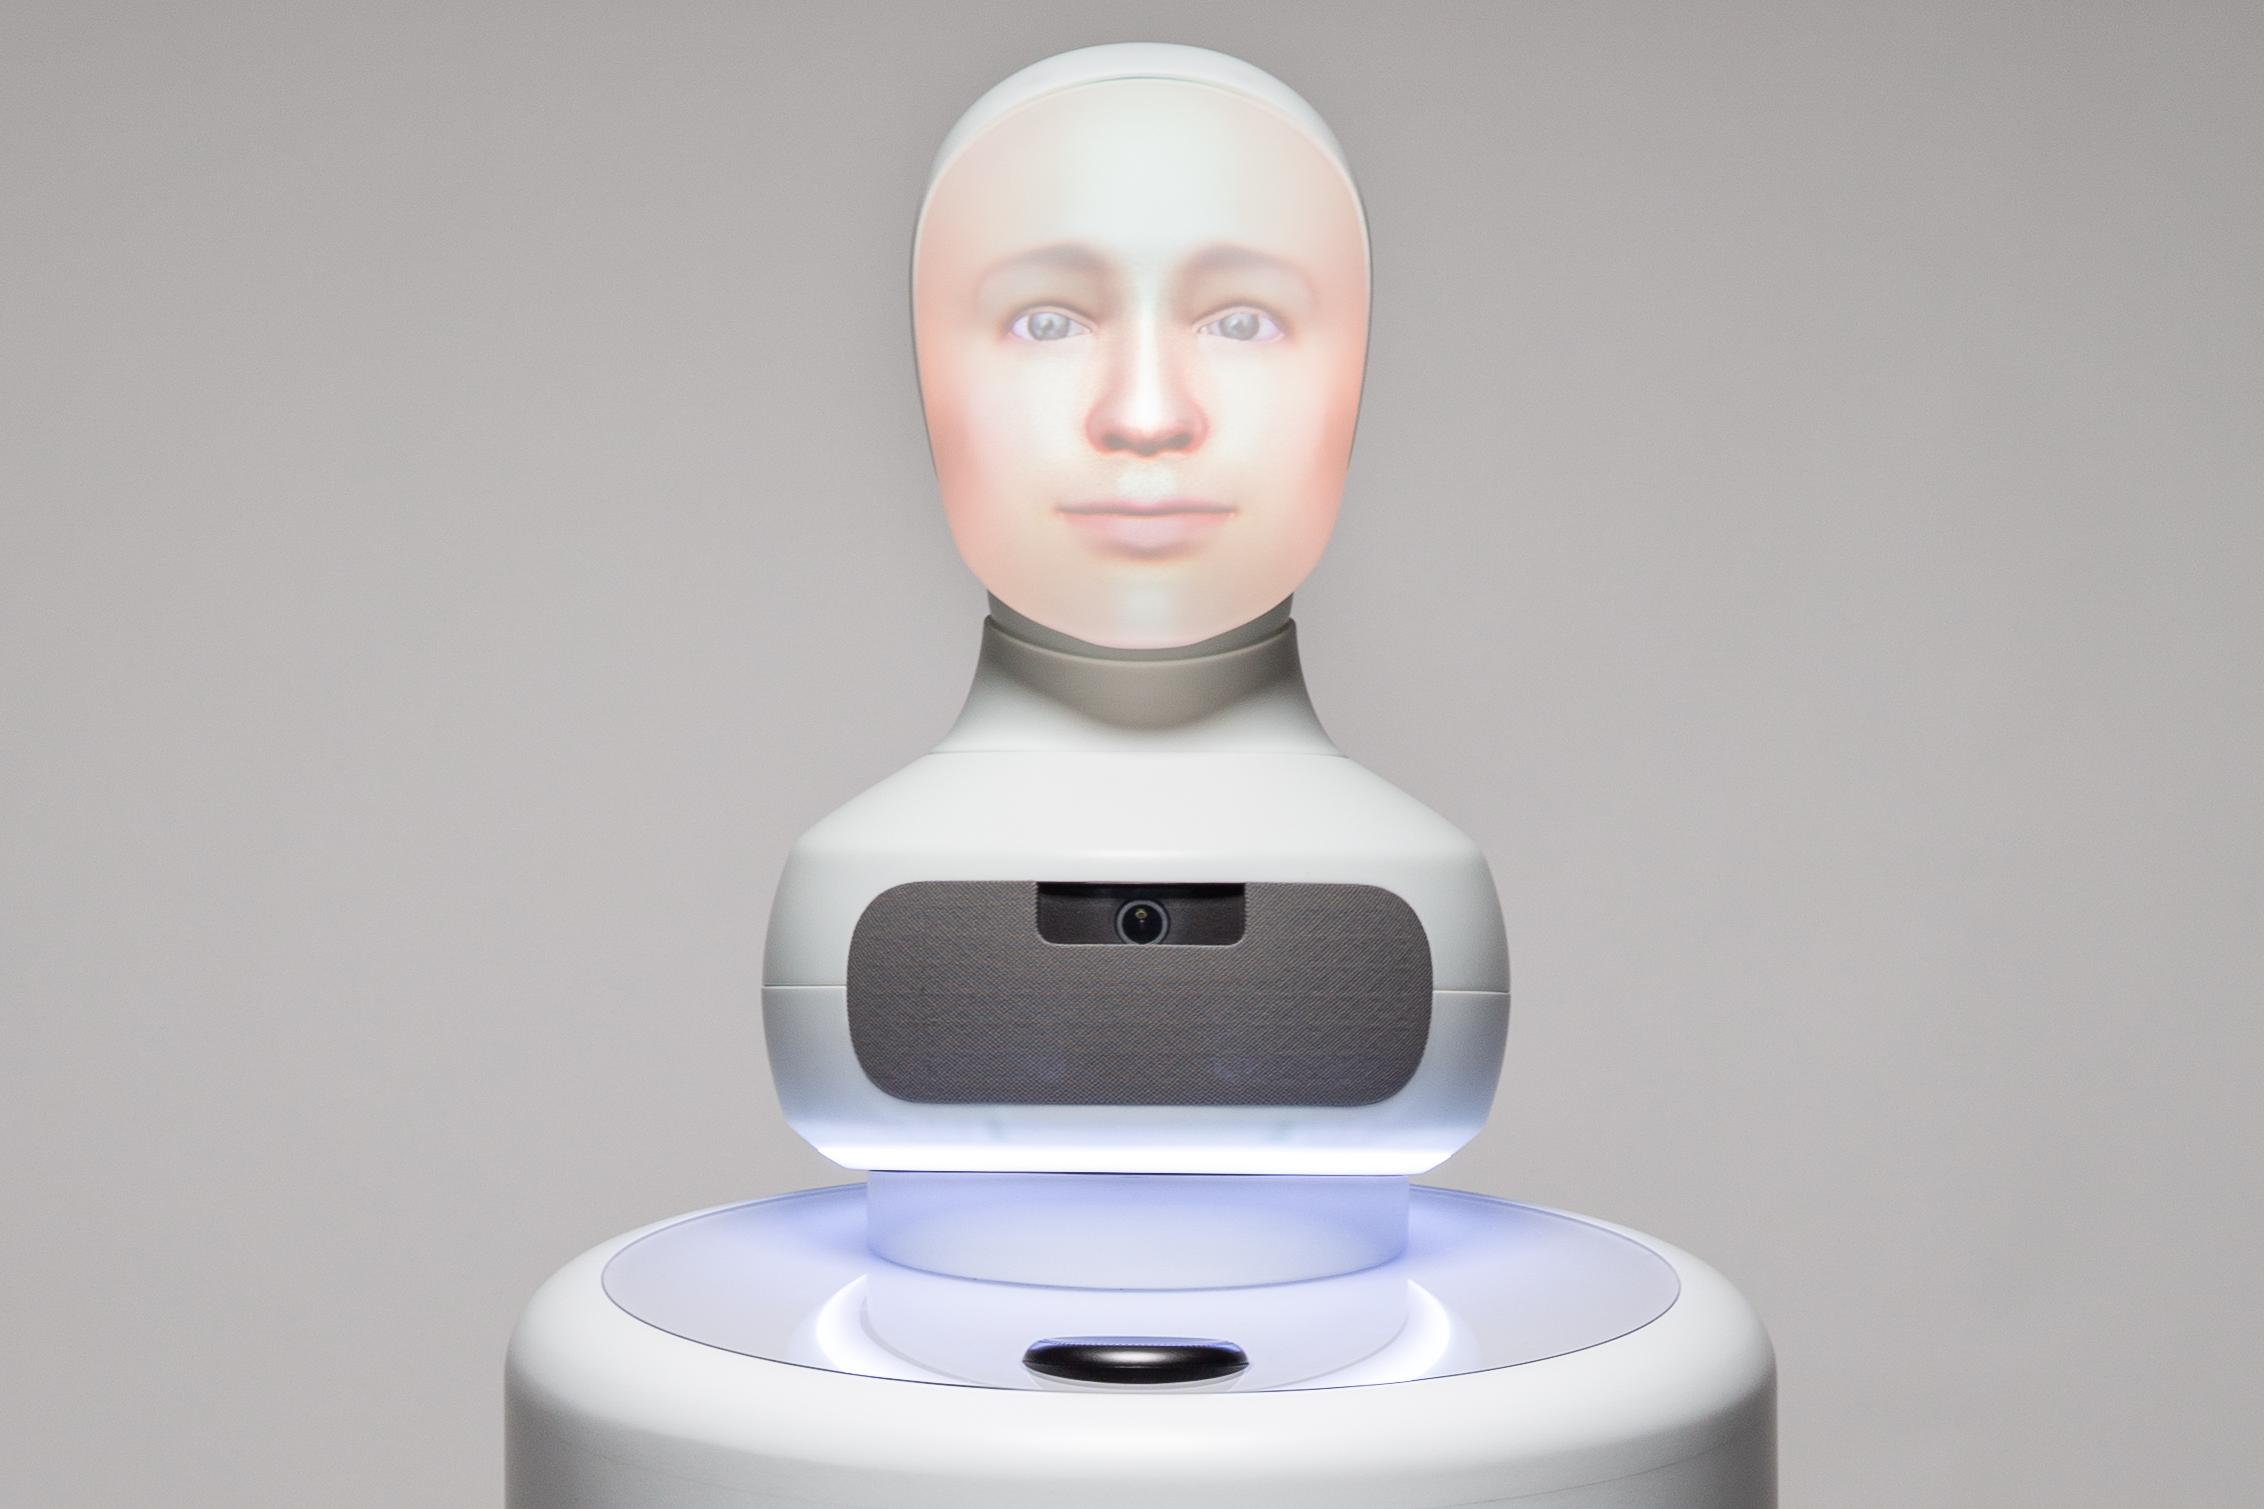
\includegraphics[width=0.26\textwidth]{graphics/study/tengai.jpg}}
 \qquad
 \subfloat[\cite{microsoft_mesh}\label{fig:image-3}]{%
      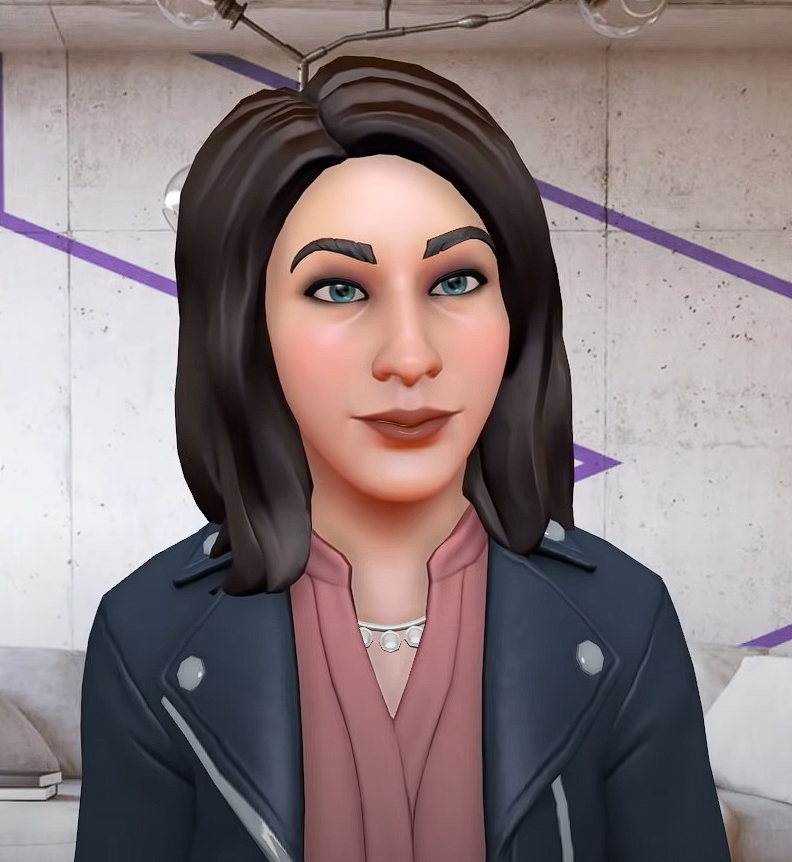
\includegraphics[width=0.26\textwidth]{graphics/study/microsoft_mesh.png}}
      
 \centering
  \subfloat[\cite{sophia}\label{fig:image-4}]{%
      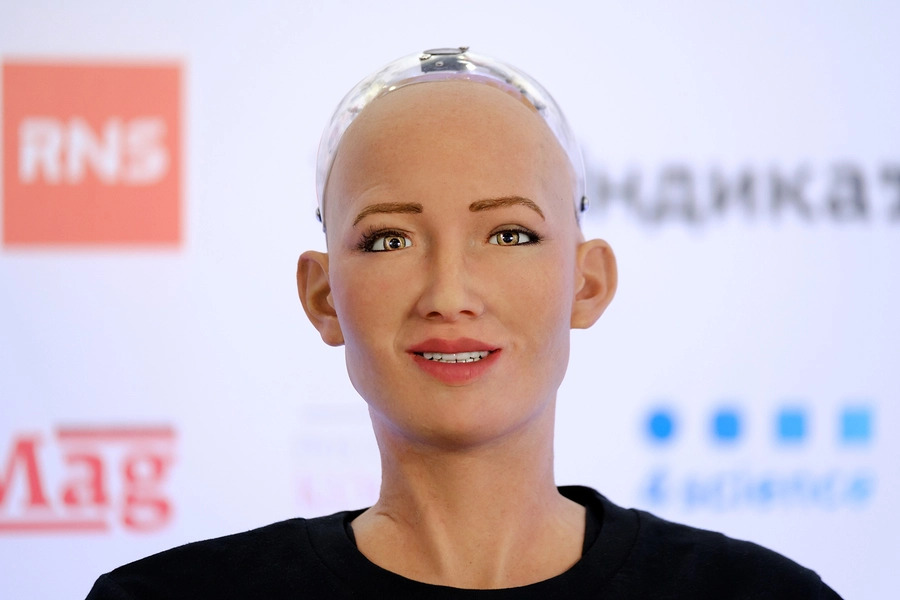
\includegraphics[width=0.26\textwidth]{graphics/study/sophia.jpg}}
 \qquad
 \subfloat[\cite{vera}\label{fig:image-5}]{%
      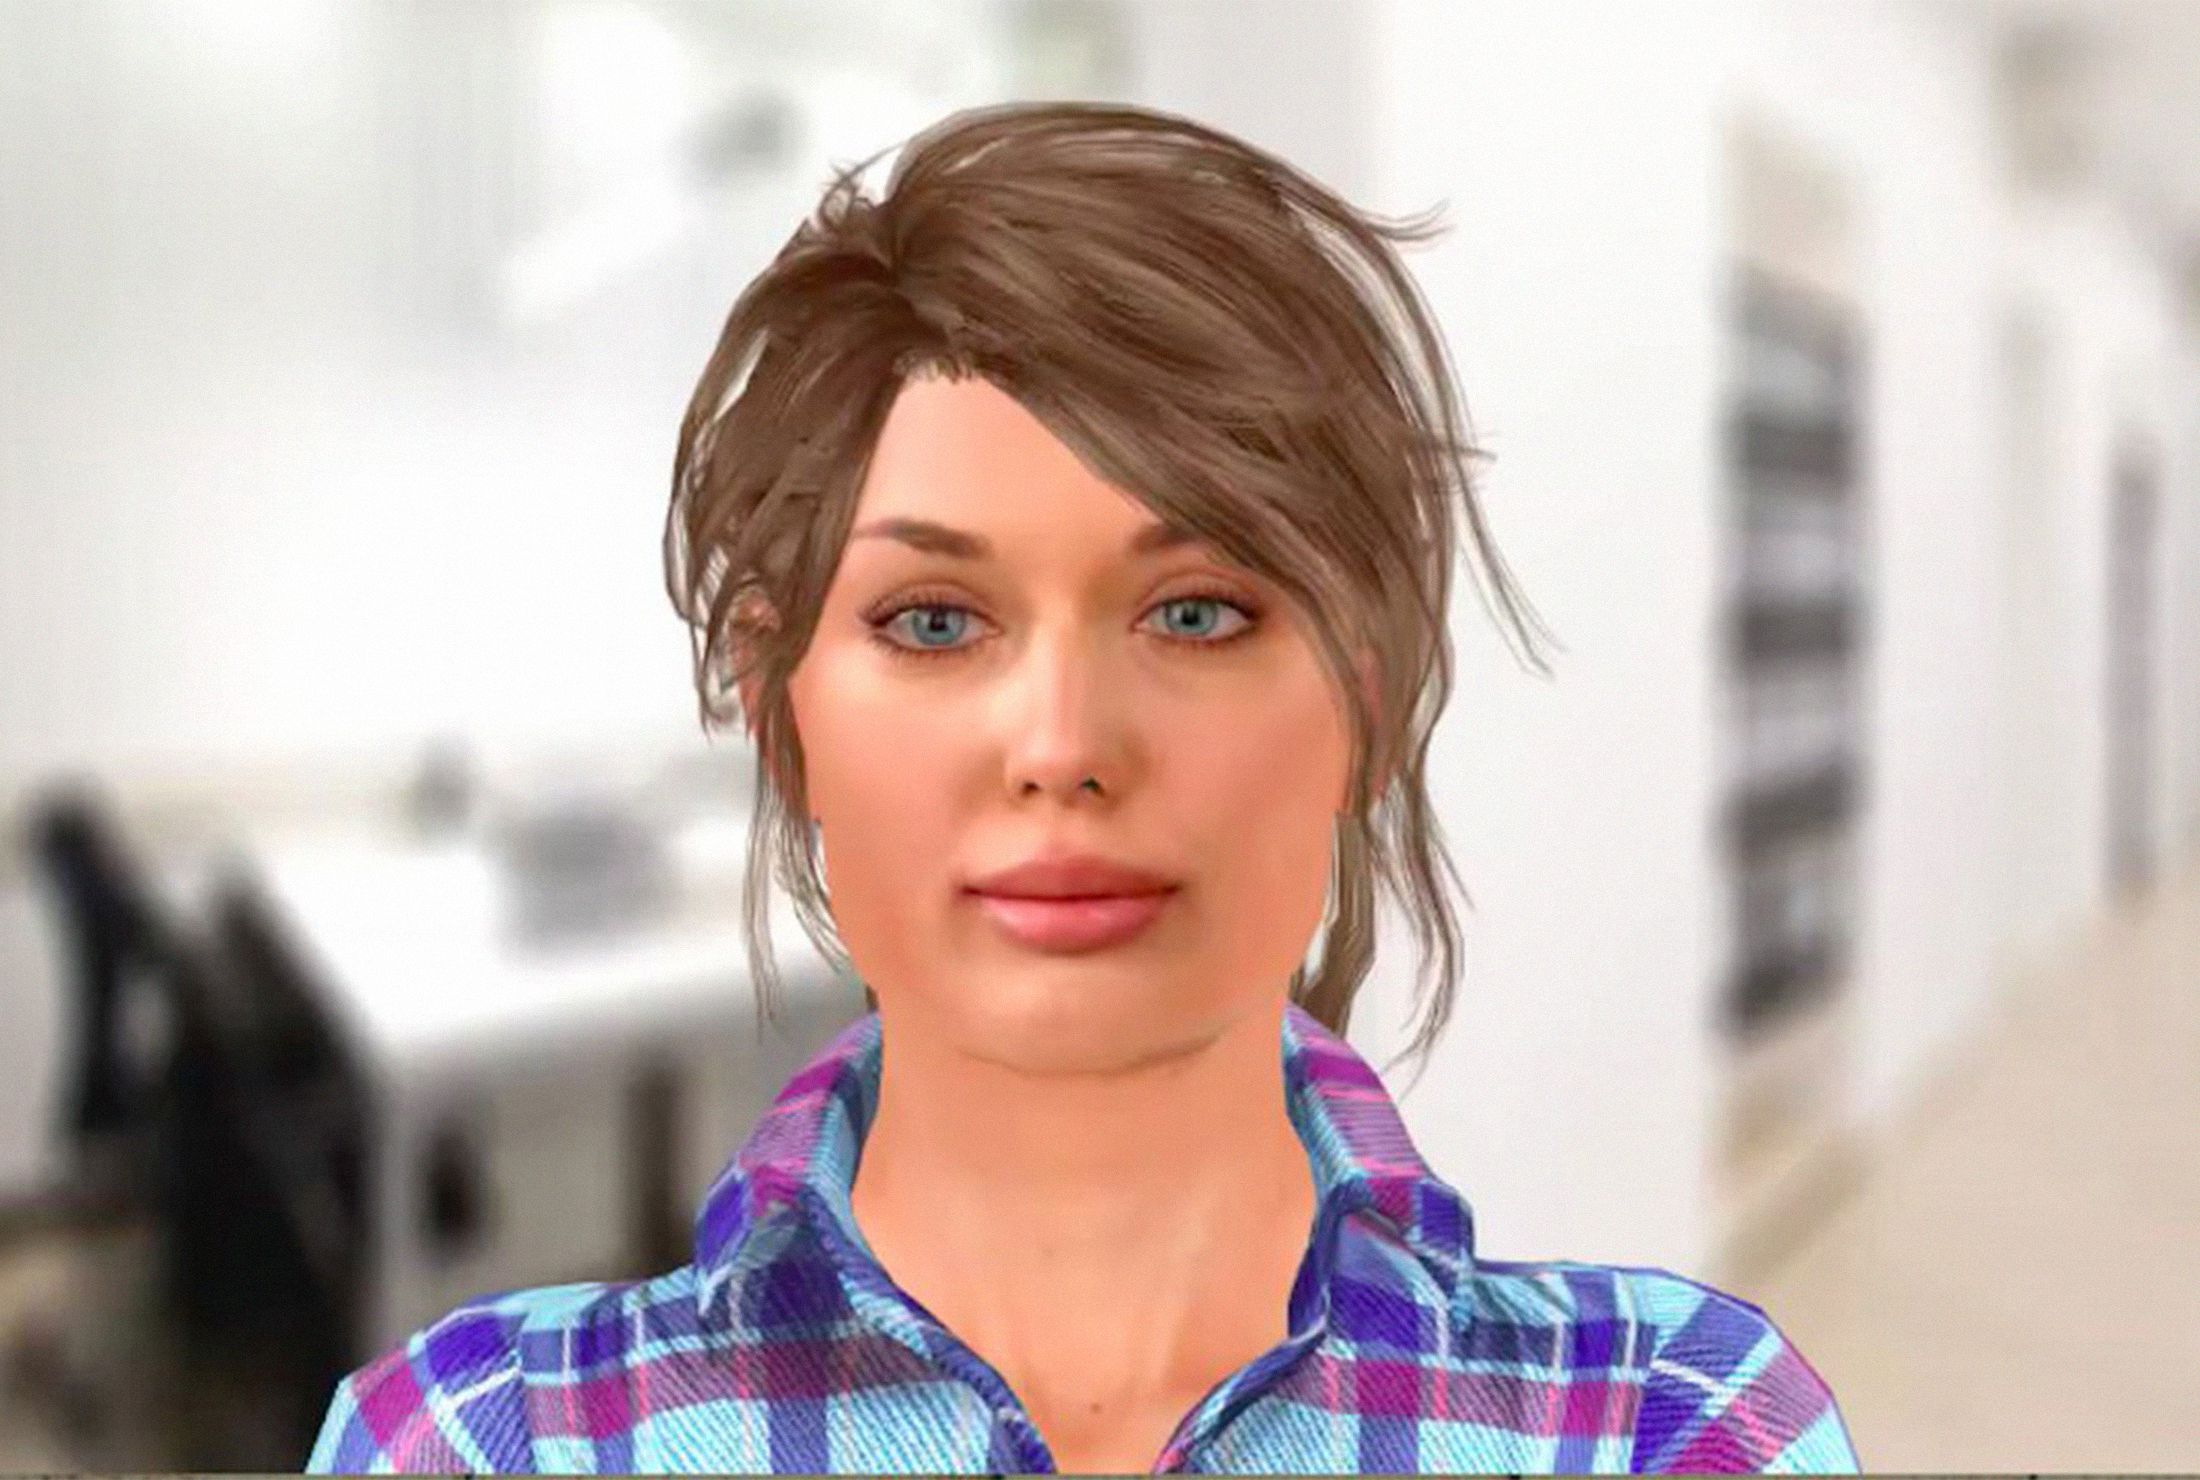
\includegraphics[width=0.26\textwidth]{graphics/study/vera.jpg}}
 \qquad
 \subfloat[\cite{facemaker}\label{fig:image-6}]{%
      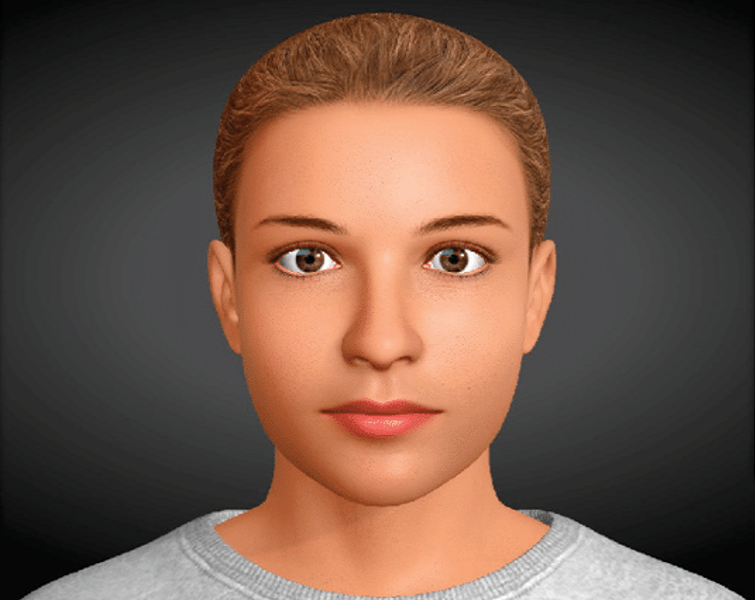
\includegraphics[width=0.26\textwidth]{graphics/study/facemaker.png}}

 \centering
 \subfloat[\cite{knoxfrost}\label{fig:image-7}]{%
      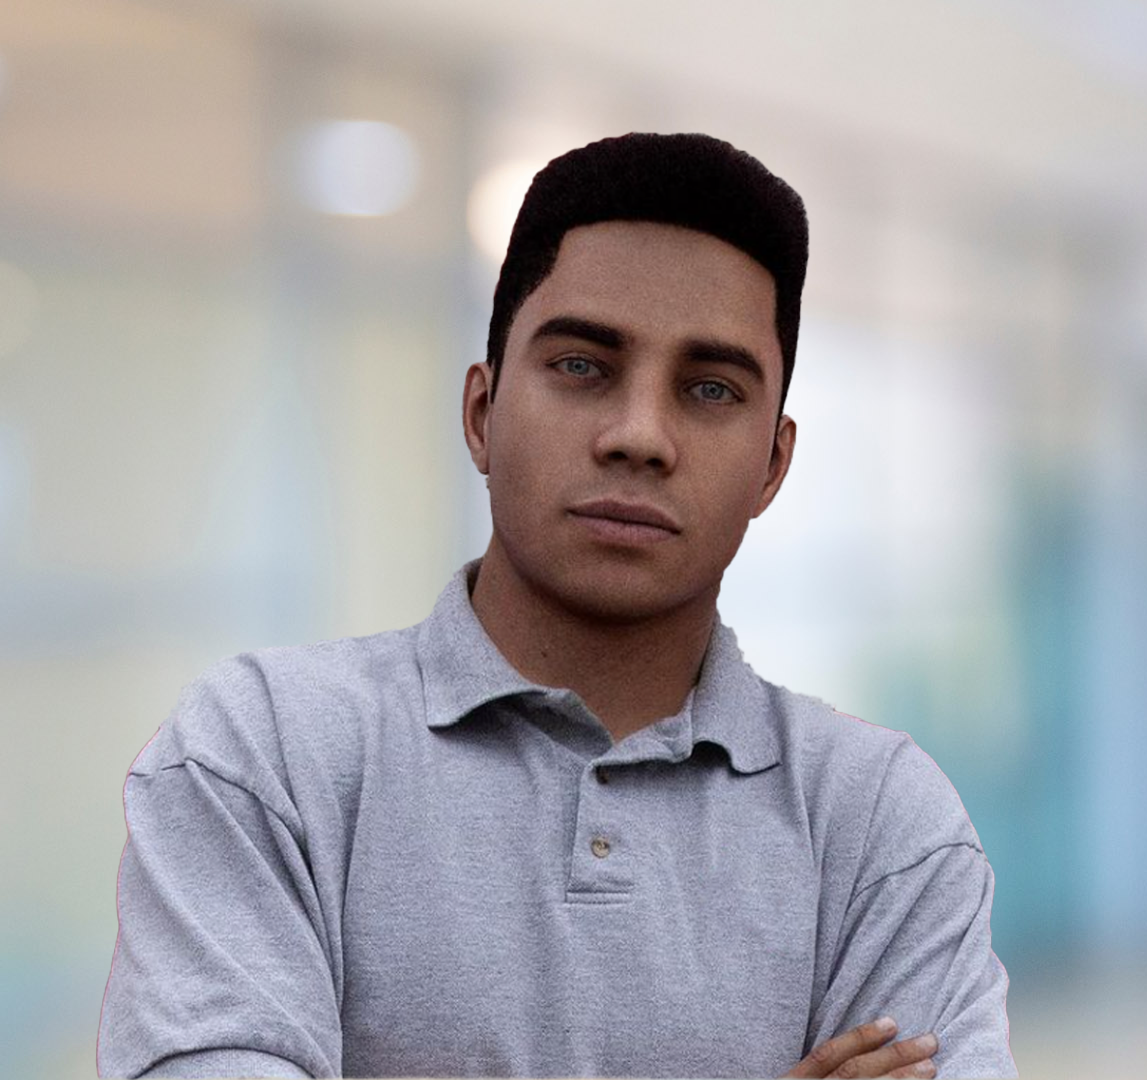
\includegraphics[width=0.26\textwidth]{graphics/study/knoxfrost.png}}
 \qquad
 \subfloat[\cite{emily}\label{fig:image-8}]{%
      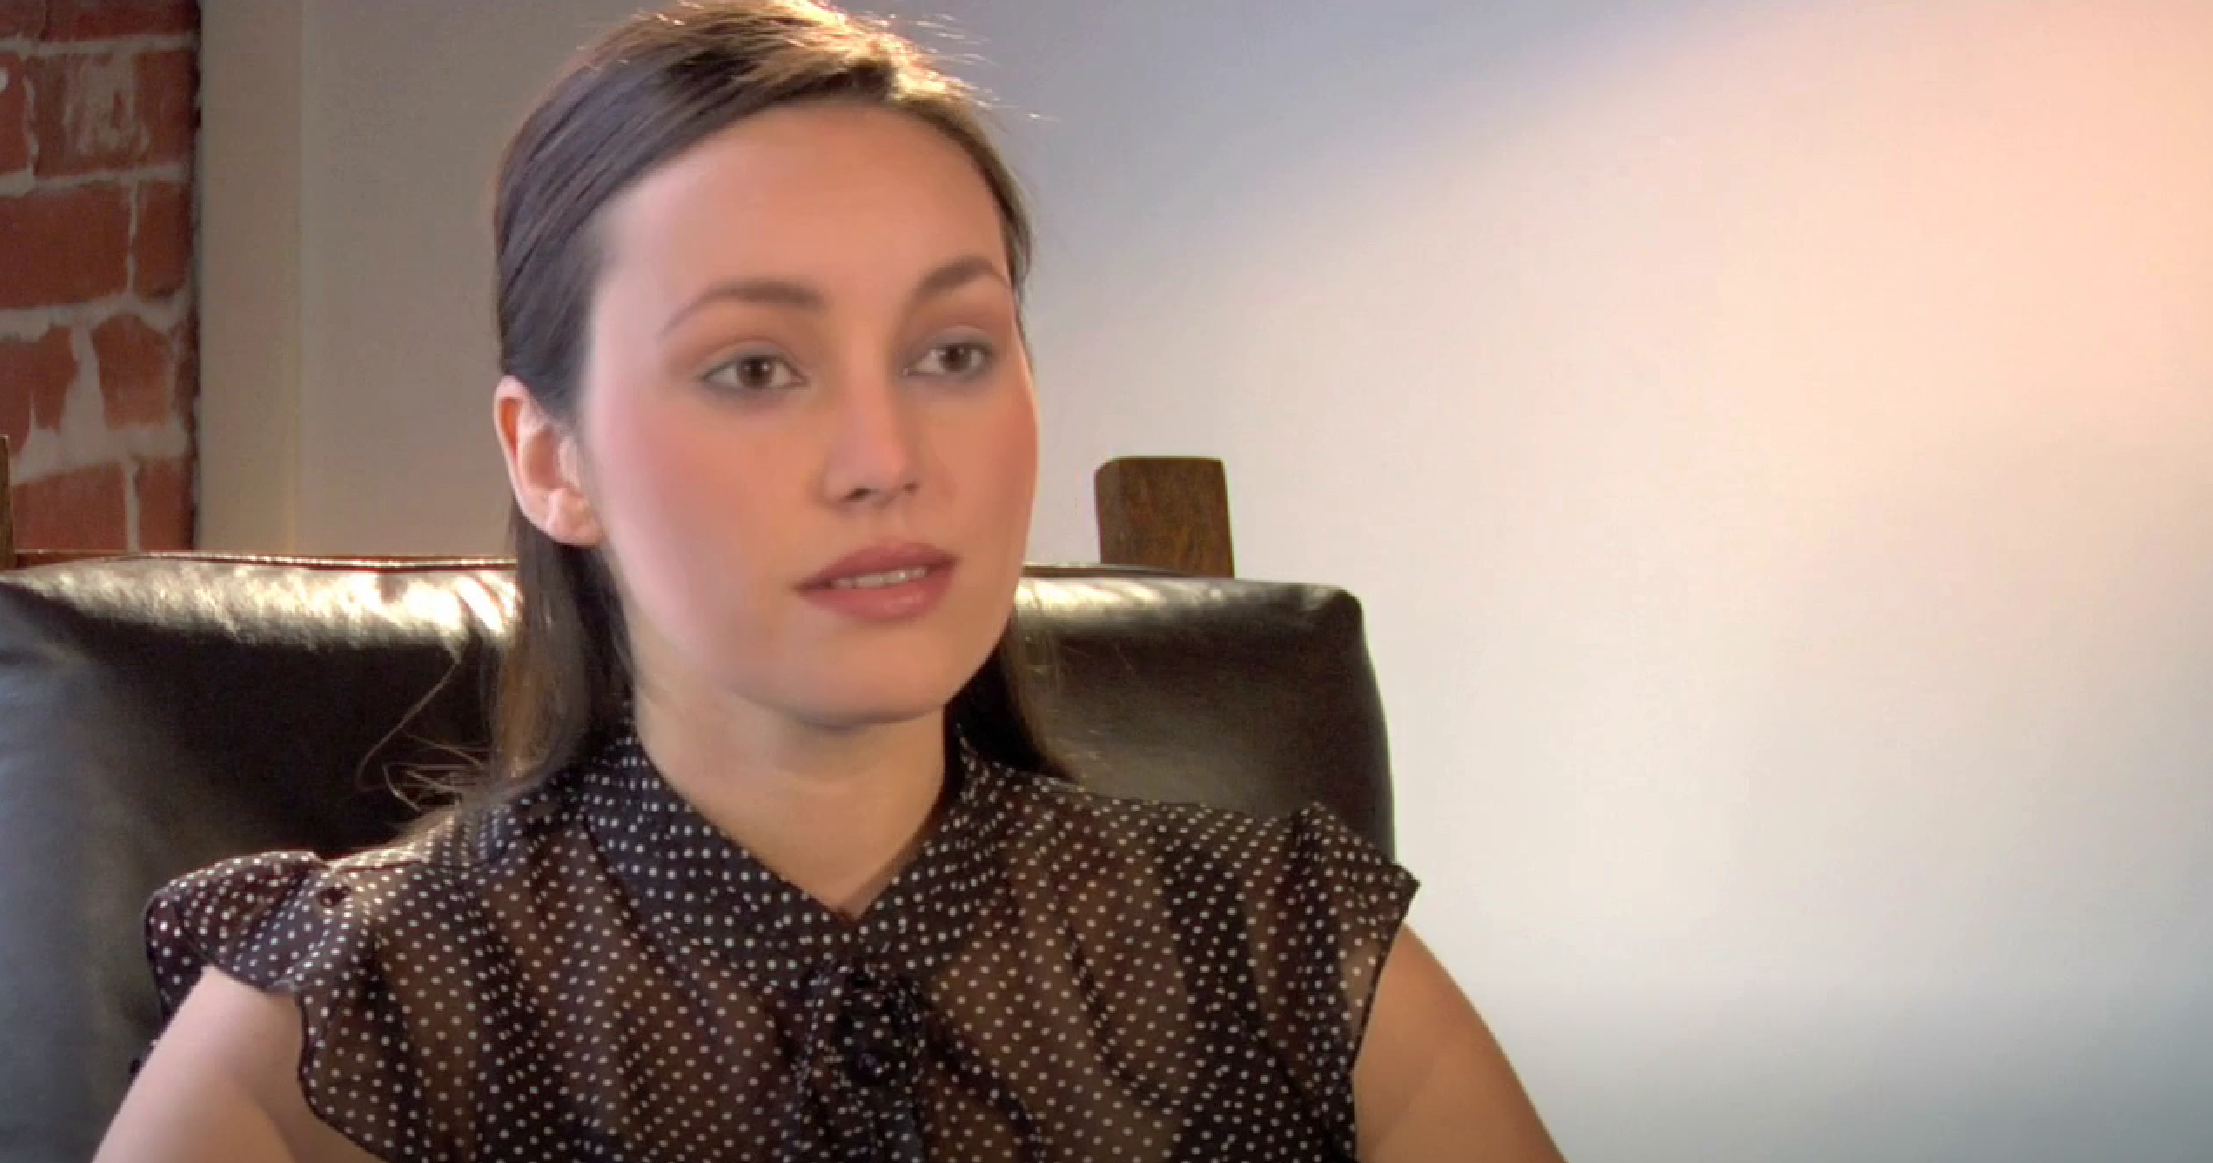
\includegraphics[width=0.26\textwidth]{graphics/study/emily.png}}
 \qquad
 \subfloat[\cite{human}\label{fig:image-9}]{%
      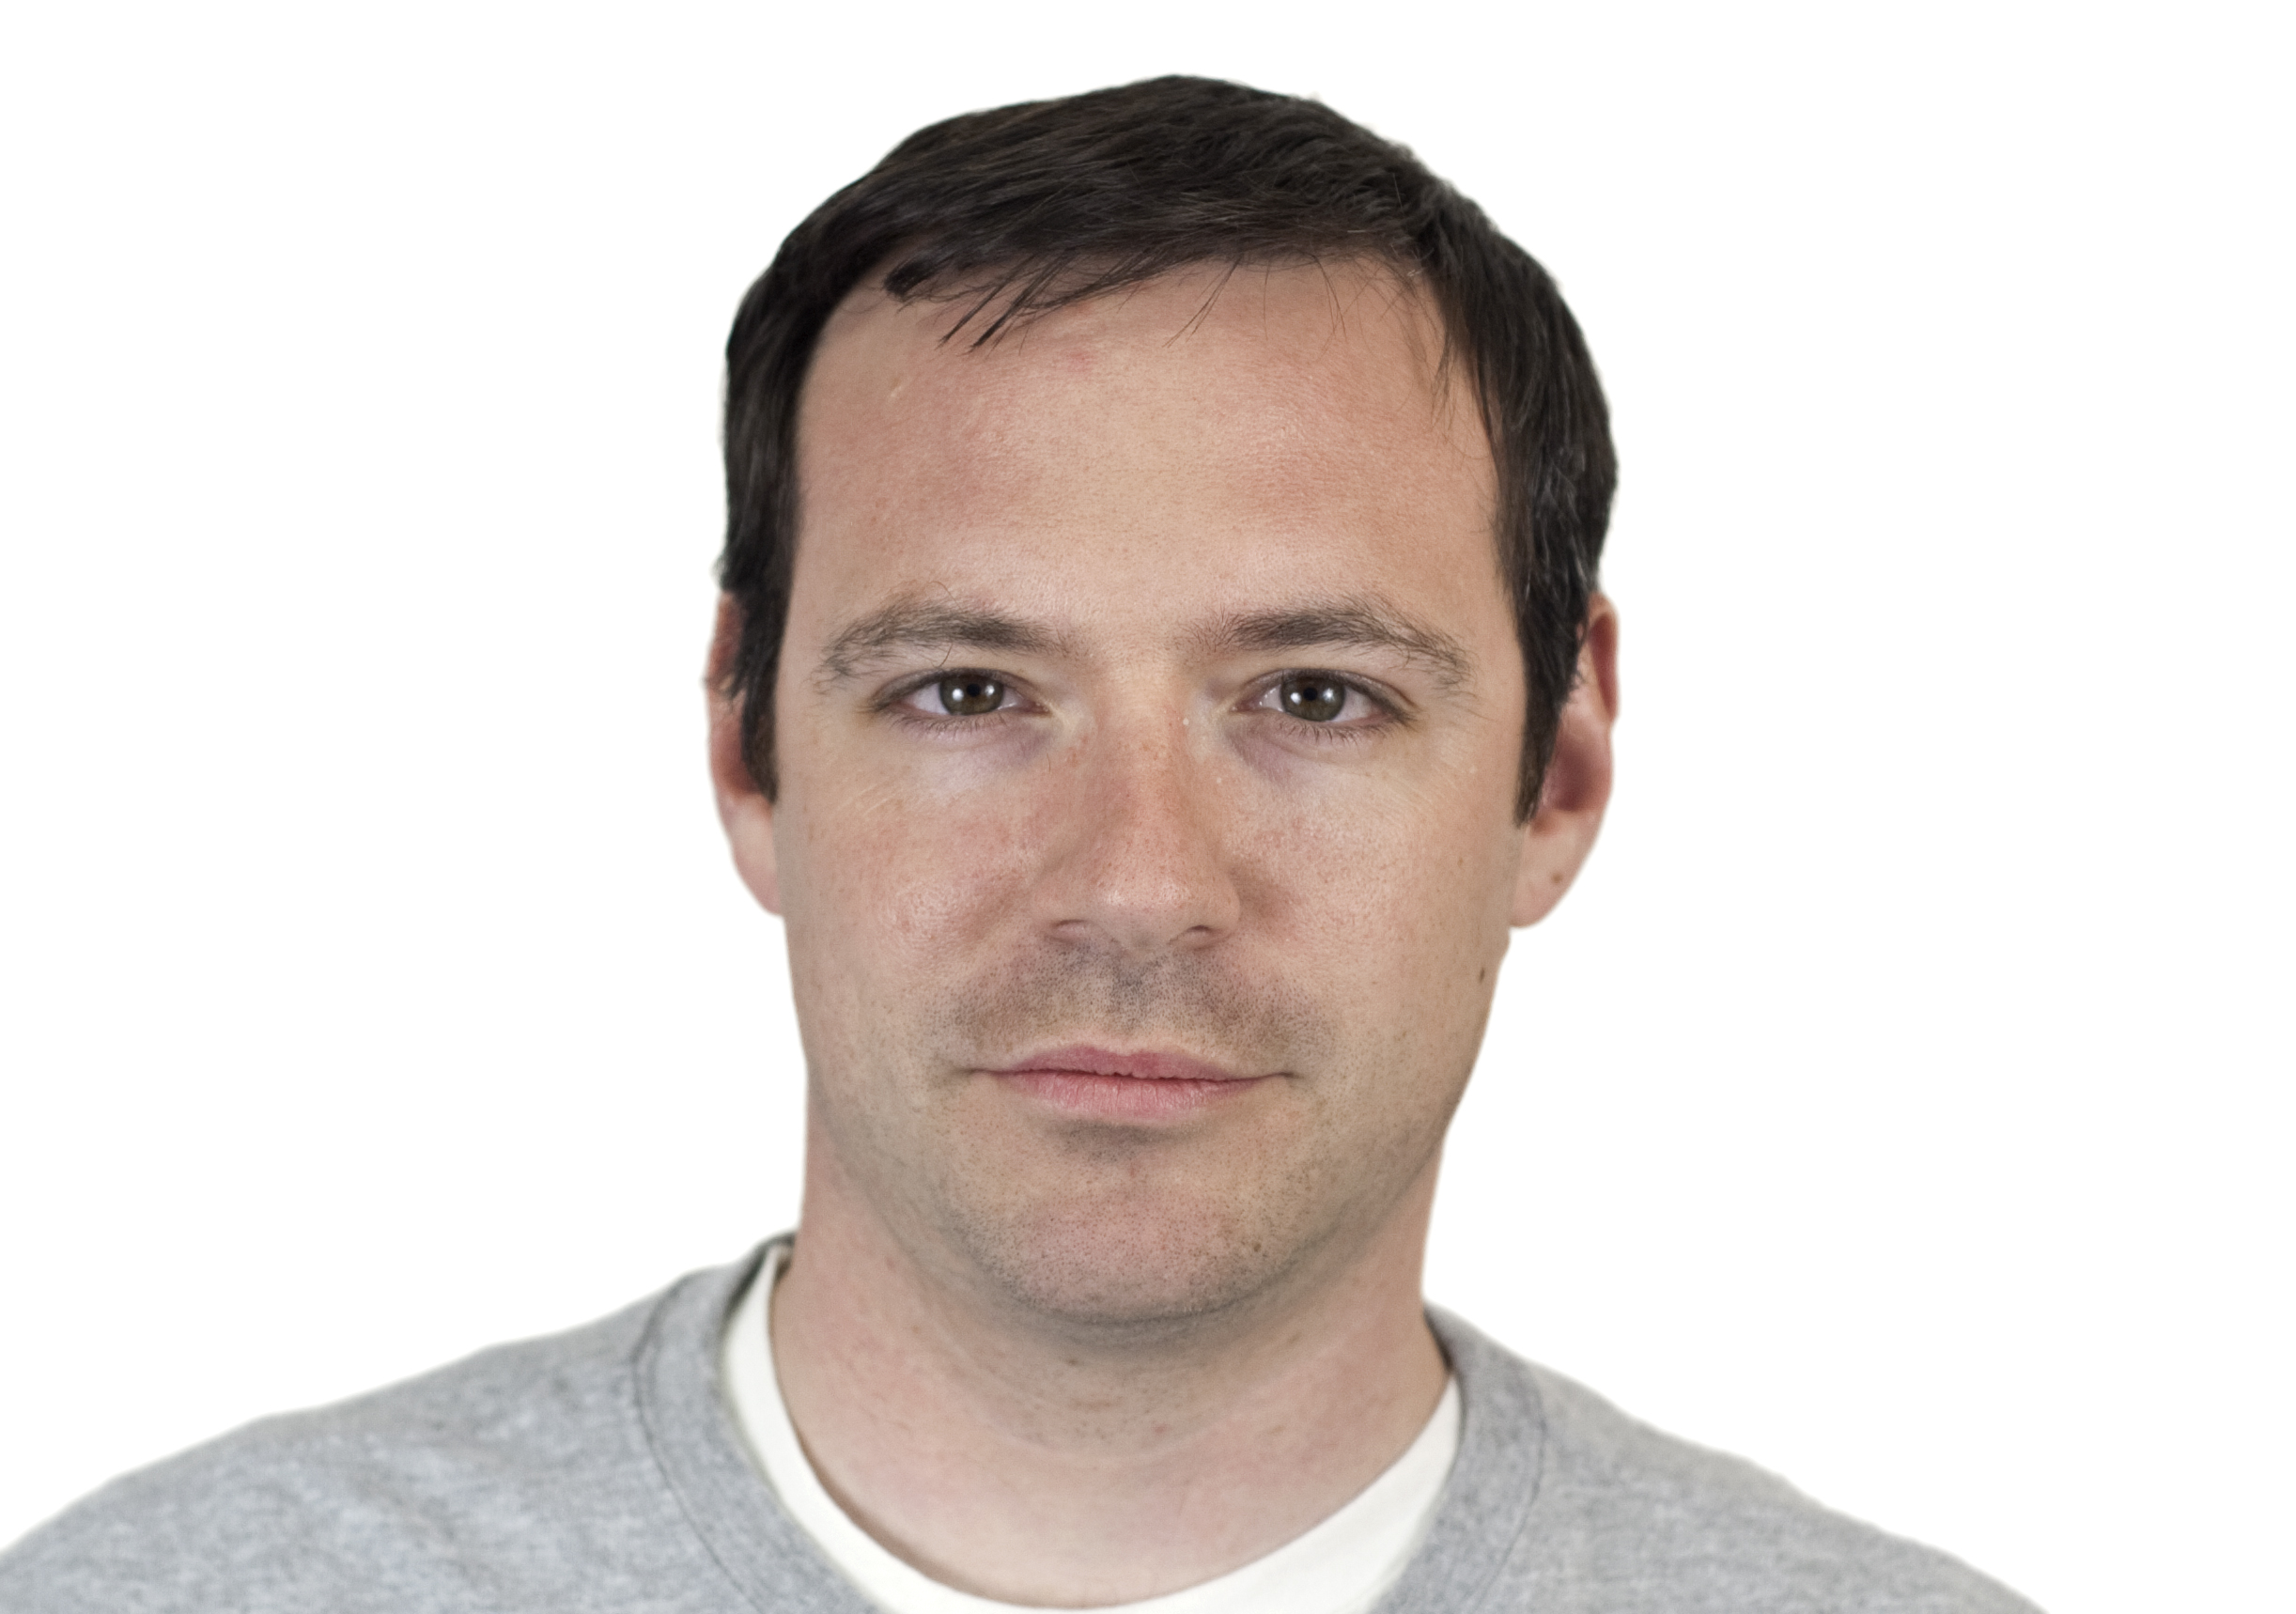
\includegraphics[width=0.26\textwidth]{graphics/study/human.jpg}}
      
\caption{The Entities used in the survey.}
\label{fig:used-entities}

\end{figure}
The focus of the pictures is on the faces of the figures, as this would also be the main focus during a job interview. Furthermore, two of the figures have atypical features. Figure \ref{fig:image-2} depicts a human face with the rest of the body being entirely mechanical, whereas Figure \ref{fig:image-4} depicts a human head with a portion of the skull missing, indicating that it is a robot.

\section{Participants}
A total of 30 people were recruited for the survey. 15 identified as  men, 12 as women, and 3 as non-binary. The age of the participants ranged from 17 to 65 years. The majority of the participants were under the age of 30, with only three over the age of 30 (ages 55 and 65), resulting in a mean age of 26.5. With a total of 27, almost all participants were from Europe, with only three from America.

\section{Method}
This research aims to assess the appearance of various robot recruiters to draw conclusions about their likeability and determine whether they fall into the uncanny valley. To do this, the participants completed a web-based questionnaire in which they had to rate eight images of possible robot recruiters with varying human-likeness and one image of a real human, as seen in Figure 6.1. Before evaluating the robot recruiters, the participants were required to read a brief introductory paragraph. In this text, the following task was described, and the participants were instructed to envision themselves at a job interview employing robot recruiting. Therefore, this introduction should place the chosen entities in the proper context for the rating task. \\
The participants had to rate each of the nine photographs individually in the evaluation assignment. For each picture, four 7-point scales between polar adjectives: mechanical/human-like, artificial/lifelike, strange/familiar and not eerie/very eerie were given. In addition, the participants had to indicate how much they liked the picture of the robot recruiter with a simple liking question. Figure \ref{fig:evaluation_task} depicts the exact appearance of the evaluation task questions. The used expressions were also translated into German for better comprehension because most participants were German speakers.
\begin{wrapfigure}[]{r}{0.65\textwidth} %this figure will be at the right
    \centering
    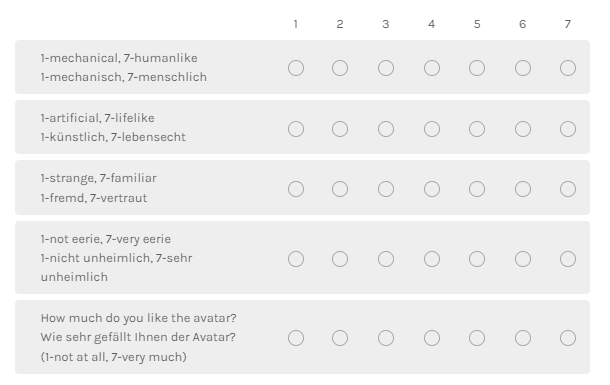
\includegraphics[width=0.65\textwidth]{graphics/evaluation_task.png}
    \caption{Questions used in the evaluation task.}
    \label{fig:evaluation_task}
\end{wrapfigure}
The first two scales (mechanical/human-like, artificial/lifelike)  have the task of inquiring about the perceived human-likeness of the figure for the participant. The other two scales (strange/familiar, not eerie/very eerie) are responsible for evaluating the participants' liking or disliking of the figures. This thesis opted to use the still commonly used term `familiar' to describe the sympathy toward the robot recruiters. To give the term `familiar' a greater significance a simple liking question (How much do you like the avatar?) was added to each assessment task of the robot recruiter. This serves to gather more evidence of the connection between familiarity toward an entity and liking an entity.\\
Before beginning the evaluation task, participants were asked to rate how much they notice the usage of computer graphics in new movies and whether they think this is a positive or negative development. Since movies often use computer-generated characters with varying degrees of human-likeness, this question was designed to assess participants' prior experience with virtual characters and the possible prior recognition of the uncanny valley.


\section{Results}
In order to make statements about the different robot recruiter figures, the mean values of the replies from the evaluation task were calculated and illustrated. In the resulting graphs, the x-axis describes the chosen robot recruiter figures, which are ordered in ascending human-likeness as comparable to figure \ref{fig:used-entities}. On the y-axis, the graphs show two or more categories of the 7-point scales, which are set side by side and analysed. The highlighted points in the graphs mark the exact mean values calculated for each figure.\par
\begin{wrapfigure}[]{r}{0.65\textwidth} %this figure will be at the right
    \centering
    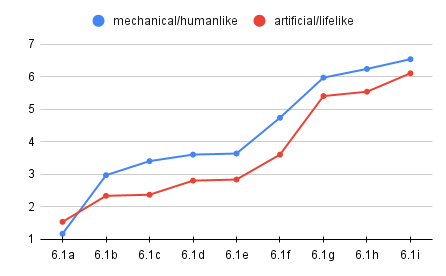
\includegraphics[width=0.65\textwidth]{graphics/result/result1.png}
    \caption{Mean values of the mechanical/humanlike and artificial/lifelike ratings of the avatars.}
    \label{fig:humanlikeness}
    \vspace{20pt}
    \centering
    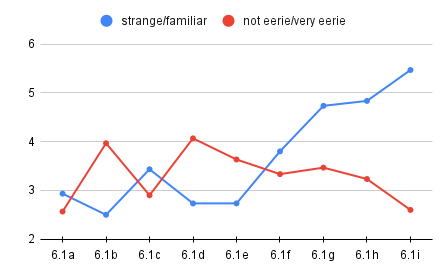
\includegraphics[width=0.65\textwidth]{graphics/result/result2.png}
    \caption{Mean values of the strange/familiar and not eerie/very eerie ratings of the avatars.}
    \label{fig:strangeness}
\end{wrapfigure}
First, the increasing human-likeness of the various entities is evaluated. Graph \ref{fig:humanlikeness} shows the mean scores of the mechanical/humanlike and artificial/lifelike scales for each selected robot recruiter avatar. In this graph, a clear link between human similarity and lifelikeness can be noticed. Furthermore, the human-likeness of the selected avatars clearly increases, as determined by the scores seen in table \ref{tab:rated-human-likeness} from the ABOT Database human-likeness predictor. The selection of the depicted robot recruiters, therefore, has been sensibly chosen for an evaluation based on increasing human-likeness.\\
Next, the relationship between the strangeness and eeriness of the characters is considered. From graph \ref{fig:strangeness}, it can be noticed that the more strange a presented robot recruiter was regarded, the eerier it was likewise rated. Equally, the more familiar a robot recruiter appeared, the less eerie it was rated. As a result, a relation between strangeness and strong eeriness, as well as familiarity and no eeriness, can be observed in the selected figures of this survey. In connection with graph \ref{fig:humanlikeness}, graph \ref{fig:strangeness} already clearly shows how the eeriness of the figures strongly decreases with a very high human resemblance. Whereas the robot recruiters in the midrange of the selected human-likenesses received varying ratings but, on average, were rated as more eerie and strange.\par
\begin{wrapfigure}[17]{r}{0.65\textwidth} %this figure will be at the right
    \centering
    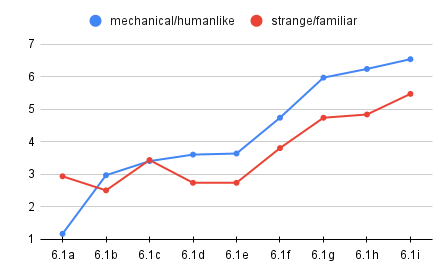
\includegraphics[width=0.65\textwidth]{graphics/result/result3.png}
    \caption{Mean values of the mechanical/humanlike and not strange/familiar ratings of the avatars.}
    \label{fig:uncanny_valley_result}
\end{wrapfigure}
Graph \ref{fig:uncanny_valley_result} shows this relation in more detail, illustrating the mechanical/humanlike and strange/familiar scales for each robot recruiter. The first thing that stands out in this graph is that the mechanical design of figure \ref{fig:image-1} was assessed with a relatively low level of familiarity. Masahiro Mori's uncanny valley hypothesis predicts that clearly categorisable robots with a moderate human resemblance would be rated with a higher familiarity. The low ranking in this study might, however, be linked to the scenario of a job interview in which the participants should imagine themselves. Since most job interviews are conducted by humans with whom you can interact and who can express emotions, a robot will lose familiarity due to the lack of these characteristics. Familiarity reduces even more with the following figure \ref{fig:image-2}, Tengai, a robot recruiter with both a human and very robot-like design. The loss of familiarity in this entity could arise with the atypical appearance. This robot recruiter combines a completely mechanical body with a very human face. This makes the entire shape of the robot difficult to categorise. This would be further supported by the low rating of figure \ref{fig:image-4}, which also has atypical features and has been rated with little familiarity despite increasing human resemblance. By contrast, the figure's \ref{fig:image-3} design shows an increasing familiarity, which can be justified by the increasing human-likeness, its unchallenging categorisation and lack of any atypical features. The next two designs, \ref{fig:image-4} and \ref{fig:image-5}, are particularly interesting. Here, a drop in familiarity with increasing human-likeness can be observed. Even though only a modest decrease in familiarity can be observed, it is significant and reminiscent of Masahiro Mori's original uncanny valley hypothesis. However, the decrease occurs with less human-likeness than expected, which can be explained by the generally very human-like characters chosen and the absence of movement, interaction or speech. With the following entity, acceptance recovers quickly and rises sharply with the following two selected recruiters. However, no chosen avatar could surpass the human. Even though the robot recruiters' likeability could not surpass that of a human, it appears that the figures \ref{fig:image-7} and \ref{fig:image-8} have escaped the uncanny valley. This could be due to a combination of the figures' nearly perfect human-like appearance and their lack of movement, and the lack of movement, which would make the non-human features stand out more.\\
In conclusion, in this study, atypical features appear to have contributed to the robot recruiters' uncanny appearance. Additionally, the entirely mechanical robot recruiter had an unexpectedly low likeability rating, which could be caused by the lack of familiarity with the use of robots during employment interviews. Finally, although the very human-like designs were able to escape the uncanny valley, no robot recruiter was able to outperform the likeability of the human recruiter.\par
With the last question of the evaluation task, asking the participants how much they liked the robot recruiters to be evaluated, this study wanted to confirm whether the participants associated the chosen term `familiarity' with the affection and liking of the robot recruiters. 
\begin{wrapfigure}[17]{r}{0.65\textwidth} %this figure will be at the right
    \centering
    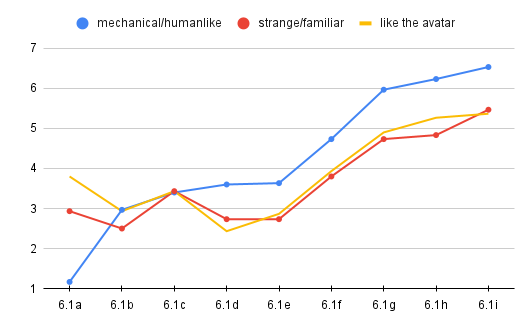
\includegraphics[width=0.65\textwidth]{graphics/result/result4.png}
    \caption{Mean values of the mechanical/humanlike, strange/familiar and liking ratings of the avatars.}
    \label{fig:likeability}
\end{wrapfigure}
Therefore, graph \ref{fig:likeability} compares the mean values of the strange/familiar and the simple liking question ratings. In addition, the graph shows the human-likeness of the avatars to illustrate their order clearly. Undoubtedly in this survey, the liking question's ratings are nearly identical to the ratings between strange and familiar. Only in the case of a purely mechanical design the character's liking is slightly greater than the familiarity rating. Overall, the ratings between strange and familiar and the liking question are almost alike, which means that in this study, a clear link can be established between the liking of a robot recruiter and its familiarity.\\
In order to better assess the participants' previous experience and personal susceptibility to the uncanny valley, two questions on the use of computer-generated graphics in films had to be answered before the robot recruiters were evaluated. Films are one of the mediums through which many people are exposed to the uncanny valley. The first question asked participants how much they noticed the use of computer graphics on a scale from 1 (very little) to 7 (very much) in films. With a mean score of 5.6, the participants in this survey noticed the use of computer graphics strongly, which speaks for a very attentive group of people with regard to the usage of virtual graphics and thus also the uncanny valley effect. The second question asked the participants whether they noticed the use of such in a positive or negative way on a scale of 1 (very negative) to 7 (very positive). With a mean score of 5.4, the participants in this study notice the use of computer graphics as a positive development. From these questions, this study theorises that most participants have already been exposed to the uncanny valley in some form in films. However, since most participants perceive the use of effects positively, it could be argued that virtual characters in films that fall into the uncanny valley are also more likely to be perceived positively by the participants. This could have had an effect on better ratings of the almost human-like robot recruiters.

\section{Discussion}
In this study, the degree of anthropomorphism of the robot recruiters had a substantial impact on their likeability. Furthermore, an uncanny valley can be recognised in the highly human-like but not entirely human-like figures \ref{fig:image-4} and \ref{fig:image-5}. However, the uncanny valley effect observed in this study is weaker than predicted in the original hypothesis by Masahiro Mori. One of the main reasons for this might be the robot recruiters' lack of movement, interaction, and voices. Moreover, contrary to Masahiro Mori's hypothesis, the completely mechanical robot recruiter was rated less likeable than expected. This could be attributable to the fact that the participants were asked to imagine the robot recruiters during a job interview. As robots are not common in employment interviews yet, this may have caused additional rejection in the participants.
Interestingly, the almost perfectly human-like robot recruiters were able to escape the uncanny valley even though they were not rated better than humans. In addition to the near-flawless human resemblance, this could also be due to the lack of movement and interaction with the robot recruiters, which would have emphasised their imperfections. 
Overall, the robot recruiters in this study with a high degree of human-likeness seem to be  associated with an increase in their likeability. Robot recruiters with a high degree of human-likeness but plainly abnormal design elements or atypical bodies, such as a combination of a mechanical and human appearance, have a low likeability and have fallen into the uncanny valley.
The mechanical robot recruiter was also rated poorly by the participants, which further speaks for the importance of a human design for robot recruiters.\\
This study was confined to a relatively small number of participants and a selected number of static images of possible robot recruiters. Furthermore, the participants' average age was quite young, and they all came from a western ethnic background. To confirm the results of this study and to increase the research on the uncanny valley in robot recruiters, the study should be repeated with a larger number of participants from diverse cultures and different age groups.
Furthermore, the integration of movement, language and possibly direct interaction with the robot recruiters would be significant factors that could lead to different evaluations of their likeability. With the likely increase in the use of robot recruiters in the coming years, further research into the interaction between robot recruiters and the impact of their appearance on their acceptance and likeability is needed. 